

\section{Intro and Whatnot}

Use \texttt{\textbackslash cref\{label\}} to get proper linked references within your document, like \cref{tab:example3}, as well as \cref{fig:example1,fig:example2}.

Standard way to use pictures can be seen in \cref{fig:example1}: 

\begin{figure}[h]
    \centering
    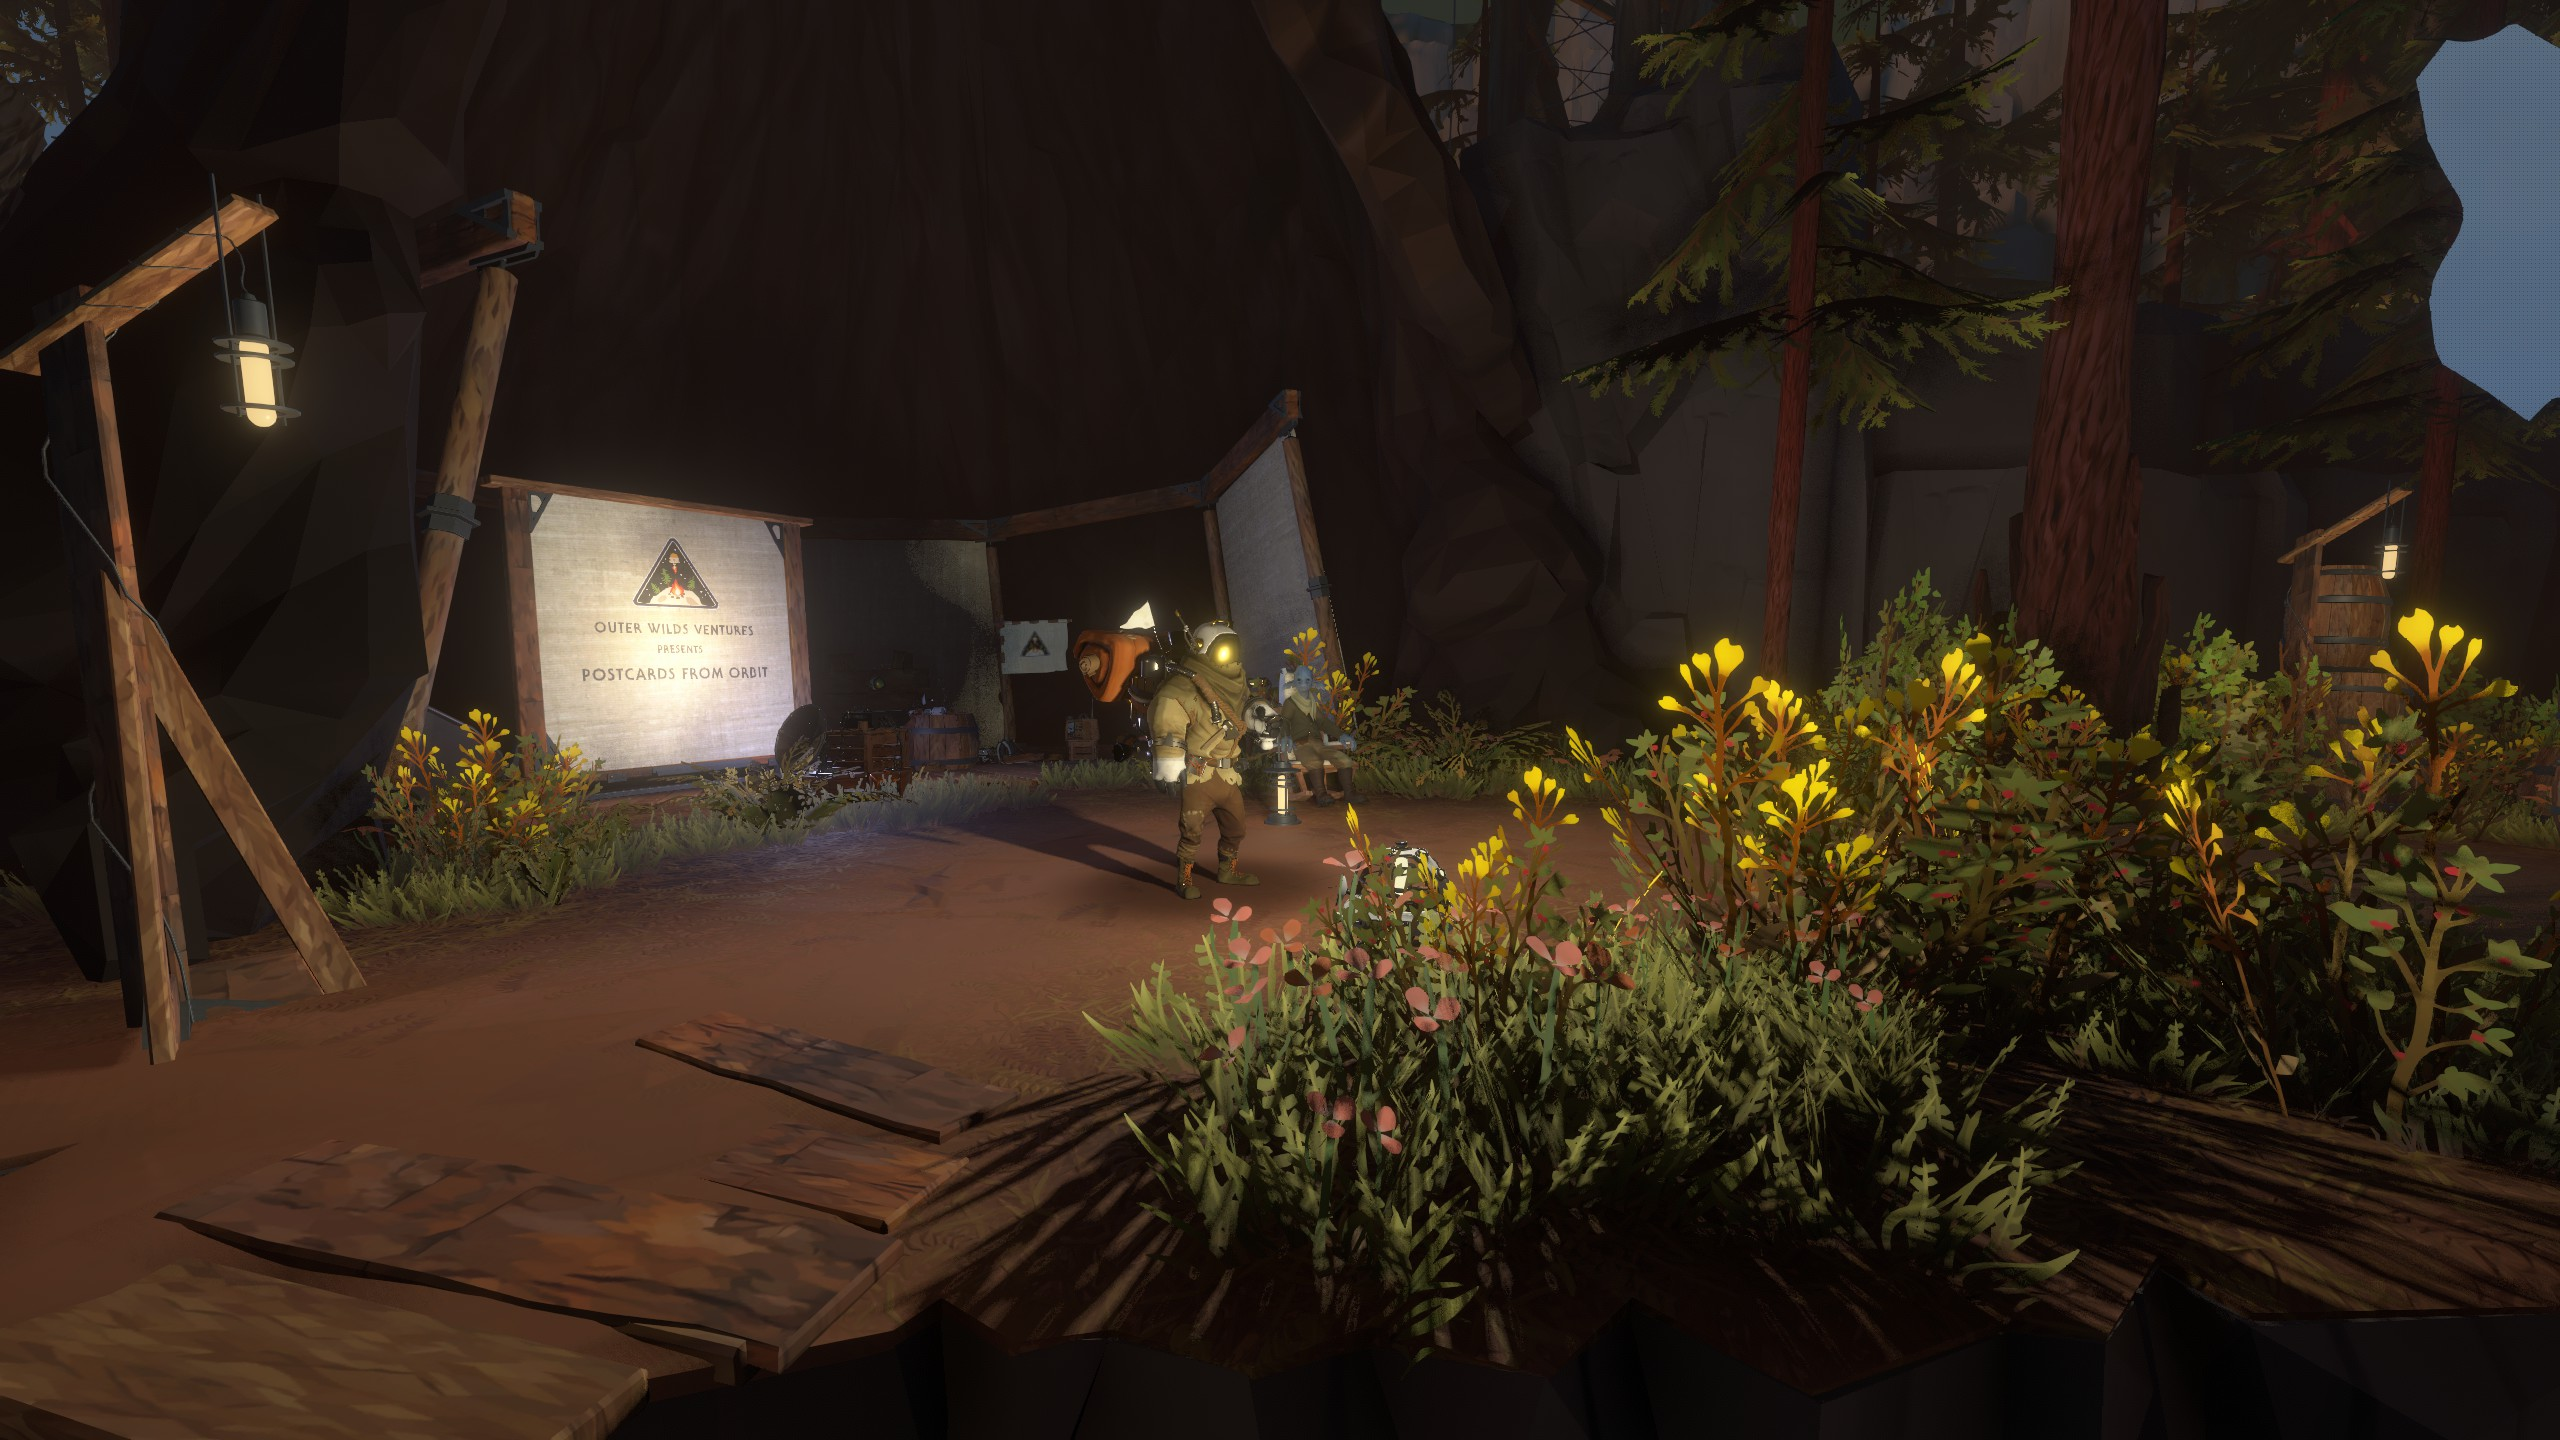
\includegraphics[width=0.7\linewidth]{images/lpbot.jpg}
    \caption{Cool pic}
    \label{fig:example1}
\end{figure}

More possibility for funky picture placements if you use TikZ:

\begin{figure}[h]
    \centering
    \begin{tikzpicture}
        \node[inner sep=0pt, draw = OWPurple, line width = 3pt] (lptop) at (-4 ,0) {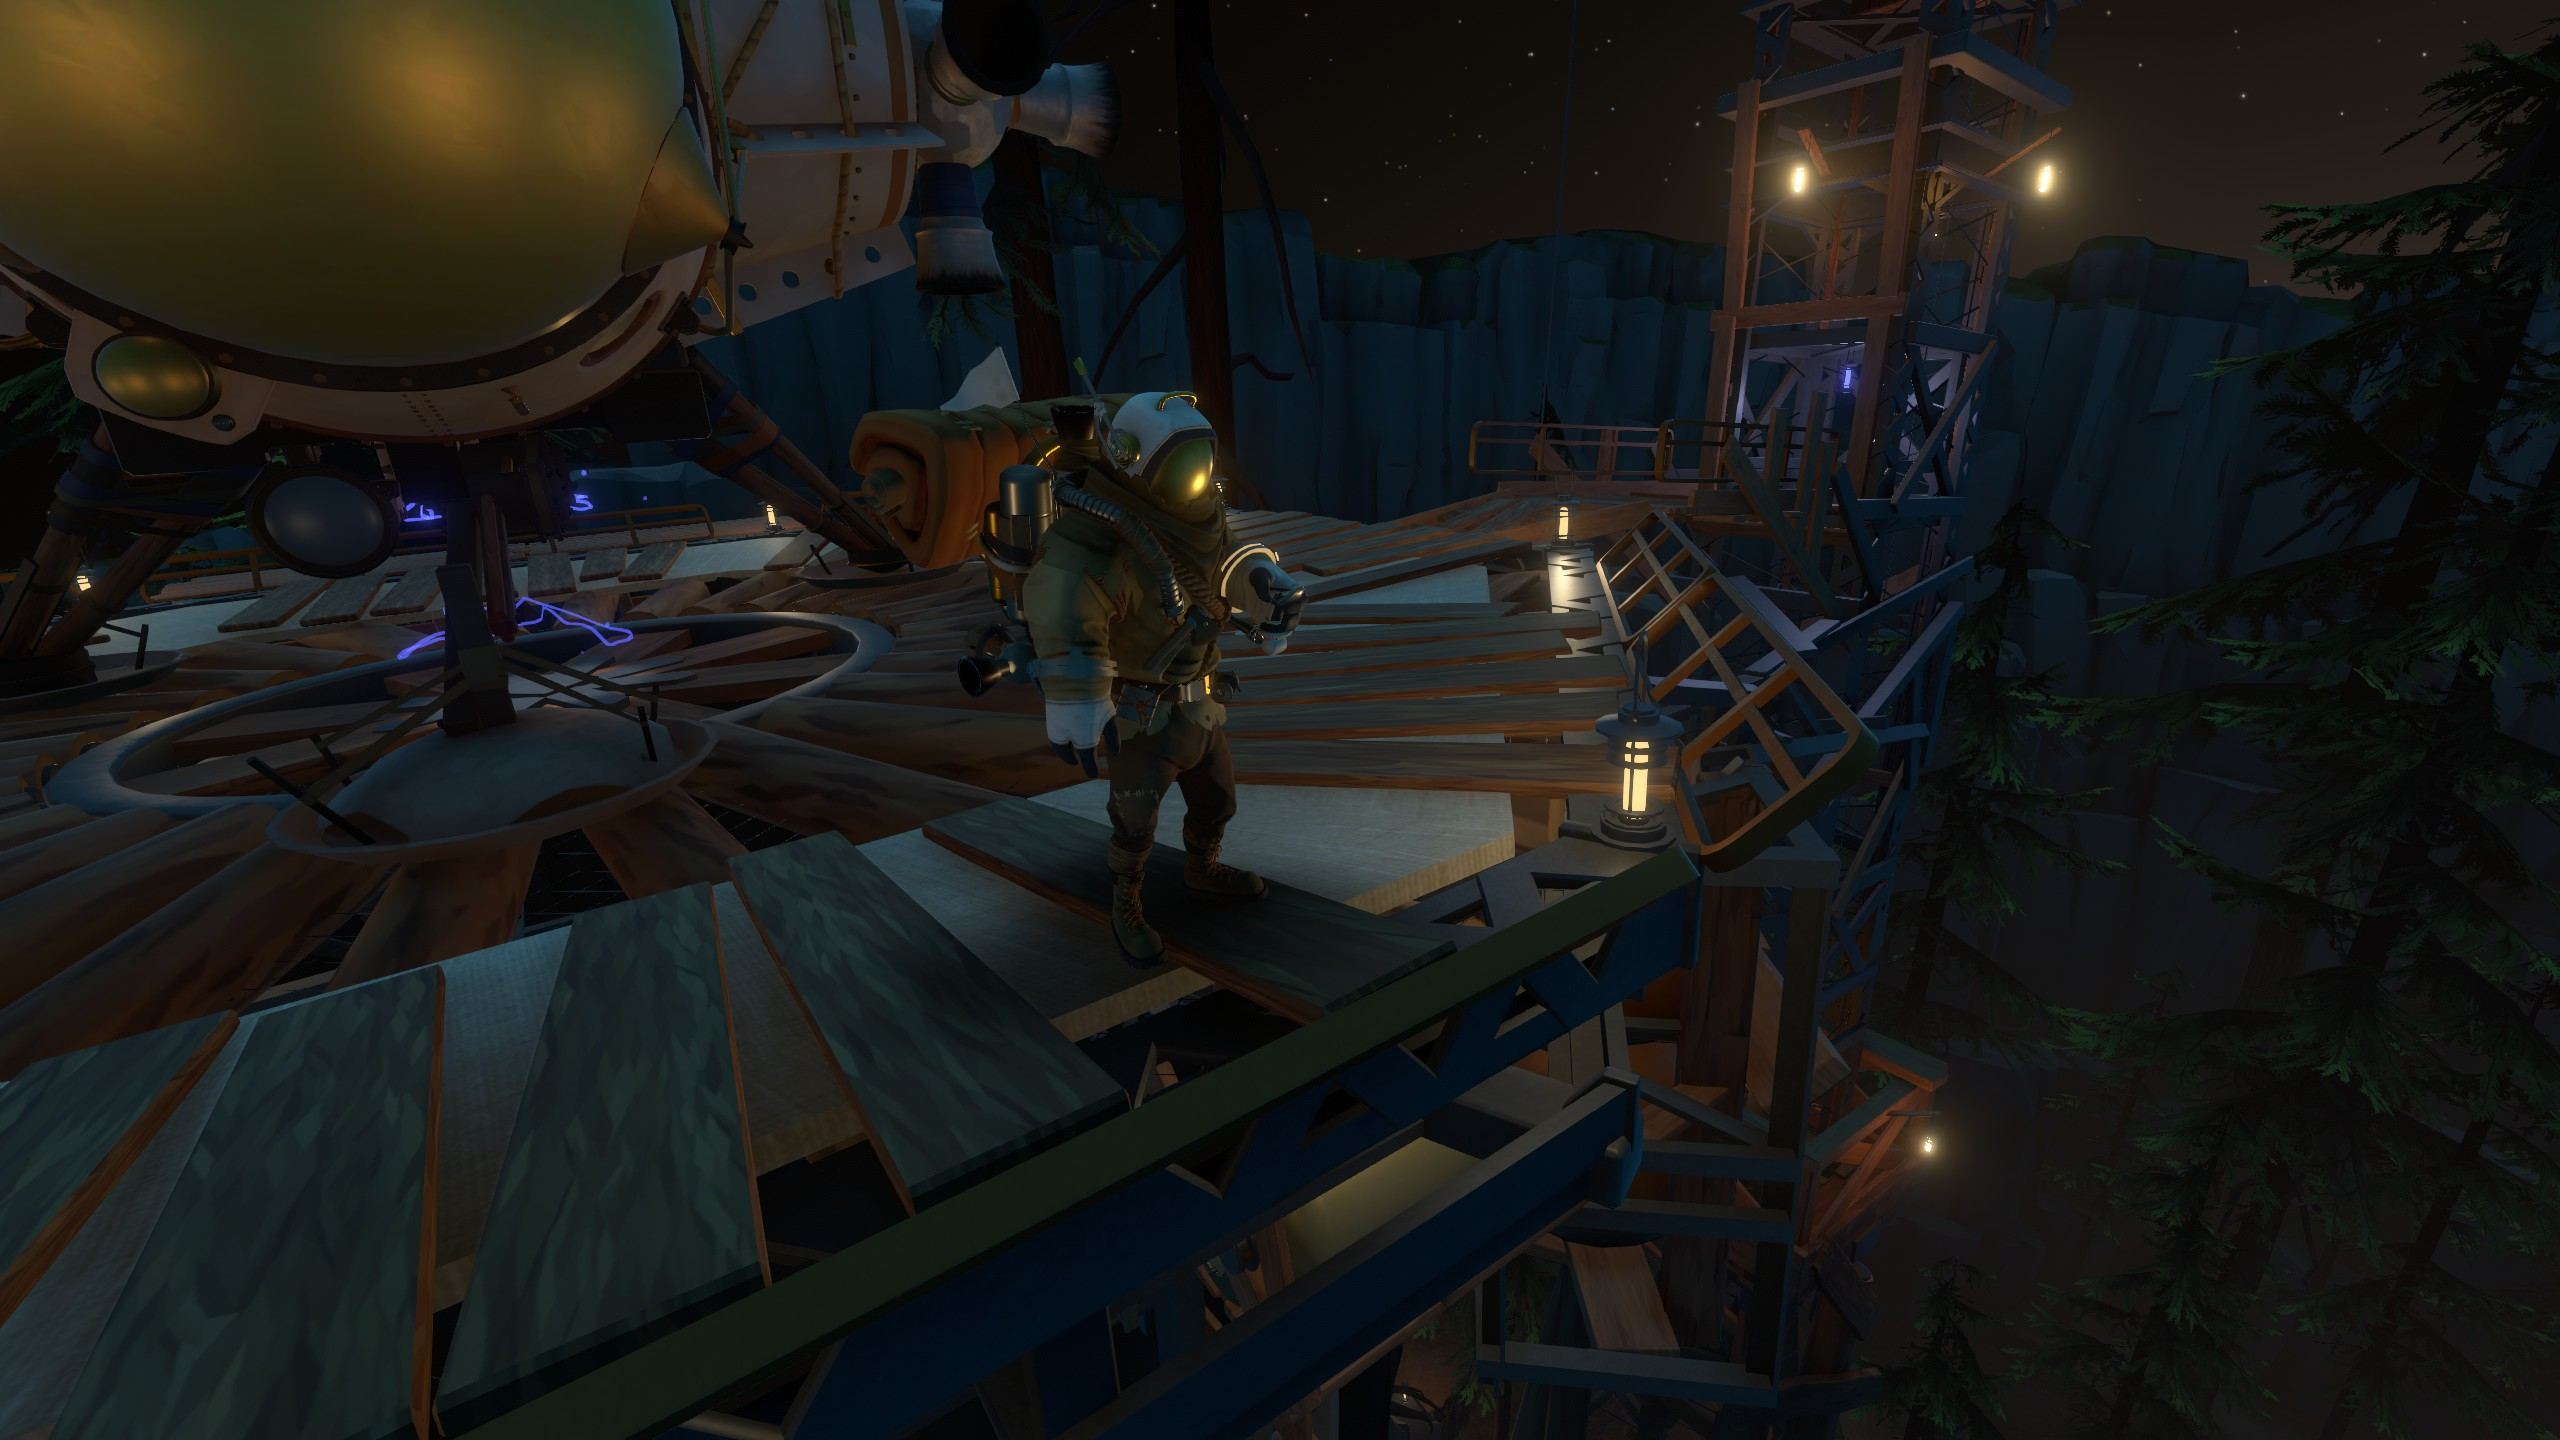
\includegraphics[width = 7.8cm]{images/lptop.jpg}};
        \node[inner sep=0pt, draw = OWBlue, line width = 7pt, rotate = 35] (mstop) at (3.5 ,0) {
\includegraphics[width = 9cm]{images/mstop.jpg}};
    \end{tikzpicture}
    \caption{Funky picture options using TikZ nodes (ignore the overfull hbox...)}
    \label{fig:example2}
\end{figure}

\clearpage

\subsection{Intro}

For consistent display of numbers with units, consider using the \texttt{\textbackslash qty\{number\}\{units\}} from the siunitx package in math-mode, displayed here:

\begin{equation}
    \sum_1^n x^2 = \qty{3.334509e21}{\meter\cubed\per\second\squared}
\end{equation}

The table style I mostly used (or some variation of this):

\begin{table}[h]
    \centering
    \caption{Super cool table}
    \renewcommand{\arraystretch}{1.3} % slightly more spacious array
    \arrayrulecolor{OWOrange} % make lines Orange
    \begin{tabular}{c c} % tabularx would allow for more customization if necessary
        \toprule
         \textbf{\color{OWOrange} Heading 1} & \textbf{\color{OWOrange} Heading Number Two} \\
         \midrule
         Stuff & Numbers \\
         Stuff & Numbers \\
         Stuff & Numbers \\
         \bottomrule
    \end{tabular}
    \label{tab:example3}
\end{table}


\subsection{Whatnot}

Behold, the colorpalette courtesy of \cite{outer_wilds_palette}:

\begin{figure}[h]
    \centering
    \begin{tikzpicture}
        \filldraw[OWGreen] (-5, 0) circle (3cm);
        \filldraw[OWOrange] (-2.5, 0) circle (3cm);
        \filldraw[OWPurple] (0, 0) circle (3cm);
        \filldraw[OWBlue] (2.5, 0) circle (3cm);
        \filldraw[OWDark] (5, 0) circle (3cm);
    \end{tikzpicture}
    \caption{Five different custom colors from the outer wilds palette, from left to right: \texttt{OWGreen, OWOrange, OWPurple, OWBlue, and OWDark}}
    \label{fig:example4}
\end{figure}

\clearpage

Using \texttt{pgfplots} allows for nifty graphs coded directly in \LaTeX \ via TikZ. It is a bit of a hassle, but sometimes worth it. 

\begin{figure}[h]
    \centering
    \begin{tikzpicture}
        \begin{axis}[xlabel={$r$ in $[\qty{}{\meter}]$},
                    ylabel={$g$  in $\left[\qty{}{\meter\per\second\squared}\right]$},
                    title={$g$ over $r$},
                    width = 14cm, 
                    height = 10cm, 
                    font = \footnotesize, 
                    legend style = {fill = black, anchor= south east, at={(0.97,.03)}}]
            \addplot[color = OWGreen, line width = 1.5pt, domain = -5:5, samples = 70]{x^2-5};
            \addlegendentry{Green};
            \addplot[color = OWBlue, line width = 1.5pt, style = dashdotted, domain = -5:5, samples = 70]{.2*x^3};
            \addlegendentry{Blue};
        \end{axis}
    \end{tikzpicture}
    \caption{Caption}
    \label{fig:example5}
\end{figure}

There is also an \texttt{ellipsebyfoci} macro in the preamble, which is useful for drawing elliptic orbits in TikZ. Stolen from \href{https://tex.stackexchange.com/questions/75017/draw-an-ellipse-from-the-two-focus-points-foci-and-the-sum-of-the-distances-fr}{here}.

